\documentclass{article}

\usepackage[margin=1in]{geometry}
\usepackage{amsmath,amsthm,amssymb}
\usepackage{bbm,enumerate,mathtools,mathrsfs}
\usepackage[hidelinks]{hyperref}
\usepackage{tikz}
\usetikzlibrary{matrix, arrows}

\newenvironment{problem}[2][Problem]{\begin{trivlist}
\item[\hskip \labelsep {\bfseries #1}\hskip \labelsep {\bfseries #2.}]}{\end{trivlist}}
\newenvironment{solution}[1][Solution.]{\begin{trivlist}
\item[\hskip \labelsep {\bfseries #1}]}{\end{trivlist}}
\newenvironment{problempart}[1]{\begin{trivlist}\item[\textbf{Part #1.}]}{\end{trivlist}}

\newenvironment{definition}[1][Definition.]{
  \begin{trivlist} \item[\hskip \labelsep {\bfseries #1}]
}{\end{trivlist}}

\newenvironment{example}[1][Example.]{
  \begin{trivlist} \item[\hskip \labelsep {\bfseries #1}]
}{\end{trivlist}}

\newenvironment{note}[1][Note.]{
  \begin{trivlist} \item[\hskip \labelsep {\bfseries #1}]
}{\end{trivlist}}

\newenvironment{theorem}[1][Theorem.]{
  \begin{trivlist} \item[\hskip \labelsep {\bfseries #1}]
}{\end{trivlist}}

\newenvironment{exercise}[1][Exercise.]{
  \begin{trivlist} \item[\hskip \labelsep {\bfseries #1}]
}{\end{trivlist}}

\newcommand{\set}[1]{\{ #1 \}}
\newcommand{\ang}[1]{\langle #1 \rangle}
\newcommand{\paren}[1]{\left( #1 \right)}
\newcommand{\fn}[3]{#1 \colon #2 \rightarrow #3}

\begin{document}

\title{Math 533: Homework 3}
\author{Peter Kagey}
\date{Wednesday, February 13, 2019}

\maketitle

% -----------------------------------------------------
% First problem
% -----------------------------------------------------
\begin{problem}{1}
\end{problem}

\begin{proof} ~
  \begin{enumerate}[(a)]
    \item The number of partitions of $n$ with no parts divisible by $d$ is
    given by the generating function \begin{align*}
      F(x)
      &= \frac{
        (1 + x + x^2 + \hdots)(1 + x^2 + x^4 + \hdots)\hdots
      }{
        (1 + x^d + x^{2d} + \hdots)(1 + x^2d + x^{4d} + \hdots)\hdots
      } \\
      &= \frac{
        \displaystyle\prod_{i=1}^\infty\sum_{j=0}^\infty x^{ij}
      }{
        \displaystyle\prod_{i=1}^\infty\sum_{j=0}^\infty x^{dij}
      }
      = \prod_{i=1}^\infty \frac{1-x^{di}}{1-x^i} \\
      &= \prod_{i=1}^\infty \paren{\frac{1}{1-x^i} - \frac{x^{di}}{1-x^i}} \\
      &= \prod_{i=1}^\infty (1 + x^i + x^{2i} + \hdots) - (x^{di} + x^{(d+1)i} + \hdots) \\
      &= \prod_{i=1}^\infty (1 + x^i + x^{2i} + \hdots + x^{(d-1)i}),
    \end{align*}
    which is identically the generating function for the number of partitions of
    $n$ with no part repeated $d$ or more times.
    \item The number of paritions of $n$ in which no part is a square is given
    by the generating function
    \begin{align*}
      F(x)
      &= \frac{
        (1 + x + x^2 + \hdots)(1 + x^2 + x^4 + \hdots)(1 + x^3 + x^6 + \hdots)\hdots
      }{
        (1 + x^1 + x^2 + \hdots)(1 + x^{4} + x^{8} + \hdots)(1 + x^9 + x^{18} + \hdots)\hdots
      } \\
      &= \frac{
        \displaystyle\prod_{i=1}^\infty\sum_{j=0}^\infty x^{ij}
      }{
        \displaystyle\prod_{i=1}^\infty\sum_{j=0}^\infty x^{i^2j}
      }
      = \prod_{i=1}^\infty \frac{1-x^{i^2}}{1-x^i} \\
      &= \prod_{i=1}^\infty \paren{\frac{1}{1-x^i} - \frac{x^{i^2}}{1-x^i}} \\
      &= \prod_{i=1}^\infty (1 + x^i + x^{2i} + \hdots) - (x^{i^2} + x^{i^2 + i} + x^{i^2 + 2i} + \hdots) \\
      &= \prod_{i=1}^\infty (1 + x^i + x^{2i} + \hdots + x^{i^2 - i}),
    \end{align*}
    which is the generating function for the number of partitions of $n$ where
    no part $j$ is repeated $j$ or more times.
    \item Here it's easy to see from the Young Diagram, and best illustrated
    with an example: \[
      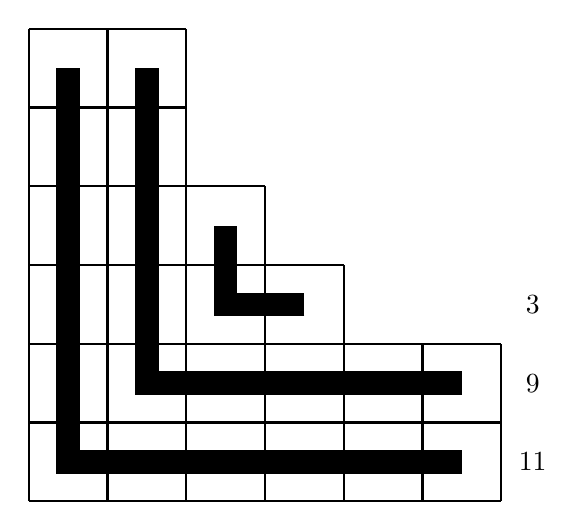
\begin{tikzpicture}
        \draw[thick]
          (0,0) grid (6,1)
          (0,0) grid (1,6)
          (1,1) grid (2,6)
          (1,1) grid (6,2)
          (2,2) grid (4,3)
          (2,2) grid (3,4)
        ;
        \draw[line width=0.3cm]
          (5.5,0.5)--(0.5,0.5)--(0.5,5.5)
          (5.5,1.5)--(1.5,1.5)--(1.5,5.5)
          (3.5,2.5)--(2.5,2.5)--(2.5,3.5)
        ;
        \node at (6.4,0.5) {11};
        \node at (6.4,1.5) {9};
        \node at (6.4,2.5) {3};
      \end{tikzpicture}
    \] Thus the self-conjugate partition $(6,6,4,3,2,2)$ is in bijection with
    the partition $(11,9,3)$.
  \end{enumerate}
\end{proof}
\pagebreak
% -----------------------------------------------------
% Second problem
% -----------------------------------------------------
\begin{problem}{2}
\end{problem}

\begin{proof} ~
  $(\Longrightarrow)$ Assume $\lambda \leq \nu$
  \\
  % This follows by a greedy algorithm. Let $ $
  $(\Longleftarrow)$
  Assume there is a sequence of partitions
  $\lambda = \mu^{(0)}, \mu^{(1)}, \hdots, \mu^{(k)} = \nu$ such that
  $\mu^{(m+1)}$ is a raise of $\mu^{(m)}$.
  \\
  By hypothesis,
  $\mu^{(m+1)} = (\mu^{(m)}_1, \hdots, \mu^{(m)}_i + 1, \hdots, \mu^{(m)}_j - 1, \hdots \mu^{(m)}_\ell)$.
  There are three cases of partial sums to consider:
  \begin{enumerate}[(i)]
    \item When the partial sums have $k < i$ terms, then
    $\mu^{(m+1)}_1 + \mu^{(m+1)}_k = \mu^{(m)}_1 + \mu^{(m)}_k$.
    \item When the partial sums have $k \geq i$ terms but fewer than $j$ terms, then
    \begin{align*}
      \mu^{(m+1)}_1 + \hdots + \mu^{(m+1)}_k
      &= \mu^{(m)}_1 + \hdots + \mu^{(m)}_i + 1 + \hdots + \mu^{(m)}_k \\
      &= \mu^{(m)}_1 + \hdots + \mu^{(m)}_k + 1.
    \end{align*}
    \item When the partial sums have $k > j$ terms, then
    \begin{align*}
      \mu^{(m+1)}_1 + \hdots + \mu^{(m+1)}_k
      &= \mu^{(m)}_1 + \hdots + \mu^{(m)}_i + 1 + \hdots + \mu^{(m)}_j - 1 + \hdots + \mu^{(m)}_k \\
      &= \mu^{(m)}_1 + \hdots + \mu^{(m)}_k.
    \end{align*}
  \end{enumerate}
  Therefore $\mu^{(m)} \leq \mu^{(m + 1)}$ and \[
    \lambda = \mu^{(0)} \leq \mu^{(1)} \leq \hdots \leq \mu^{(k)} = \nu,
  \] and so $\lambda \leq \nu$.
\end{proof}
\pagebreak
% -----------------------------------------------------
% Third problem
% -----------------------------------------------------
\begin{problem}{3}
\end{problem}

\begin{proof}
\end{proof}
% -----------------------------------------------------
% Fourth problem
% -----------------------------------------------------
\begin{problem}{4}
\end{problem}

\begin{proof} ~
  \begin{enumerate}
    \item There are $n!$ ways to linearly order $[n]$. Then partitioning into
    sizes of $(1^{a_1}, 2^{a_2}, \hdots k^{a_k})$ within each cycle of size $n$ there
    are $n$ equivalent ways to pick the first element. Similarly, if there are
    $a_i$ cycles of size $i$, there are $a_i!$ equivalent ways to arrange the
    cycles. Thus there are \[
      \frac{n!}{
        \underbrace{1 \cdots 1}_{a_1} \cdot
        \underbrace{2 \cdots 2}_{a_2} \cdots
        \underbrace{k \cdots k}_{a_k}
        a_1! a_2! \cdots a_k!
      } = \frac{n!}{z_\lambda}
    \]
    \item
    Let $S_n$ act on itself by conjugation. It is sufficient to compute the size
    of the stabilizer of $w$, \[
      \operatorname{Stab}(w)
      = \set { \sigma \in S_n : \sigma w \sigma^{-1} = w}
      = \set{ \sigma \in S_n : \sigma w = w \sigma },
    \]
    and the orbit is \[
      \mathcal O(w) = \set{\sigma w \sigma^{-1} : \sigma \in S_n}.
    \]
    Since conjugation preserves cycle type, $\mathcal O(w)$ consists of all
    elements of cycle type $\lambda$ and $\#\mathcal O(w) = n!/z_\lambda$, as
    above.
    Then by the orbit-stabilizer theorem, \[
      \#\operatorname{Stab}(w)
      = \frac{\#S_n}{\#\mathcal O(w)}
      = \frac{n!}{n!/z_\lambda}
      = z_\lambda,
    \] as desired.
  \end{enumerate}
\end{proof}
\pagebreak
% -----------------------------------------------------
% Fifth problem
% -----------------------------------------------------
\begin{problem}{5}
\end{problem}

\begin{proof} ~
\end{proof}
\pagebreak
% -----------------------------------------------------
% Six problem
% -----------------------------------------------------
\begin{problem}{6}
\end{problem}

\begin{proof} ~
  \begin{enumerate}[(a)]
    \item
    % Let $\Gamma$ be an element of the subspace generated by
    % $p_1, p_3, p_5, \hdots$.
    % It is sufficient to show that the generators are
    Notice that if $f_1, f_2 \in \bigoplus_n \Gamma^n$, then
    $f_1f_2 \in \bigoplus_n \Gamma^n$ and $f_1 + f_2 \in \bigoplus_n \Gamma^n$.
    Thus in order to show that an element of $\Gamma$ is in $\bigoplus_n \Gamma^n$,
    it is sufficient to show that the generators $p_1, p_3, p_5, \hdots$ are in
    $\bigoplus_n \Gamma^n$.
    \\
    Clearly $p_{2i-1} \in \Gamma^{2i-1}$, and furthermore, \begin{align*}
      p_{2i-1}(x_1, -x_1, x_3, x_4, \hdots)
      &= x_1^{2i-1} + (-x_1)^{2i-1} + x_3^{2i-1} + x_4^{2i-1} + \hdots \\
      &= x_3^{2i-1} + x_4^{2i-1} + \hdots \\
      &= p_{2i-1}(x_3, x_4, \hdots).
    \end{align*}
    Next it is necessary to show that any element of $\bigoplus_n \Gamma^n$ can
    be written as a sum of products of odd power sum symmetric functions.

    \item Since the power sum symmetric functions are multiplicative, it is
    sufficient to show that the number of partitions of $n$ into
    distinct parts is equal to the number of partitions into odd parts.
    This is easy enough to show by generating function trickery.
    The generating function for partitions into distinct parts is given by
    \begin{align*}
      (1 + x)(1 + x^2)(1 + x^3)\cdots
      &= \frac{1-x^2}{1-x}\cdot\frac{1-x^4}{1-x^2}\cdot\frac{1-x^6}{1-x^3}\cdots \\
      &= \frac{1}{1-x}\cdot\frac{1}{1-x^3}\cdot\frac{1}{1-x^5}\cdots \\
      &= (1 + x + x^2 + \hdots)(1 + x^3 + x^6 + \hdots)(1 + x^5 + x^{10} + \hdots)\cdots,
    \end{align*}
    which is the generating function for partitions into odd parts.
  \end{enumerate}
\end{proof}
\end{document}
